%%%%%%%%%%%%%%%%%%%%%%%%%%%%%%%%%%%%%%%%%
% Practical 1 CS181
%%%%%%%%%%%%%%%%%%%%%%%%%%%%%%%%%%%%%%%%%

%----------------------------------------------------------------------------------------
%	BASIC PACKAGES AND DOCUMENT CONFIGURATIONS
%----------------------------------------------------------------------------------------

\documentclass{article}

\usepackage[version=3]{mhchem} % Package for chemical equation typesetting
\usepackage{siunitx}  				 % Provides the \SI{}{} and \si{} command for typesetting SI units
\usepackage{graphicx} 				 % Required for the inclusion of images
\usepackage{natbib}   				 % Required to change bibliography style to APA
\usepackage{amsmath}  				 % Required for some math elements 
\usepackage[left=2.0cm,top=1.6cm,right=2.0cm,nohead,nofoot]{geometry} % Set margins
\usepackage[section]{placeins}
\usepackage{amsfonts}
\usepackage{booktabs}
\usepackage{array}
\usepackage{hyperref}
\setlength{\footskip}{20pt}  % Distance of page number to text
\setlength\parindent{0pt} % Removes all indentation from paragraphs
\renewcommand{\labelenumi}{\alph{enumi}.} % Make numbering in the enumerate environment by letter rather than number (e.g. section 6)

%\usepackage{times} % Uncomment to use the Times New Roman font

%----------------------------------------------------------------------------------------
%	REPORT HEADER
%----------------------------------------------------------------------------------------
\title{\vspace{-1.0cm}Stuff}
\title{Predicting Photovoltaic Efficiencies of Molecules} % Title

\author{Authors: Taylor Names, Samuel Kaplan and David Castineira} % Author name
\date{\vspace{-5ex}}  % Remove date
\begin{document}

\maketitle % Insert the title, author and date


%----------------------------------------------------------------------------------------
%	SECTION: INTRODUCTION
%----------------------------------------------------------------------------------------

\section*{Introduction}

The fundamental objective of this project is to use machine learning techniques to predict the potential efficiency of organic photovoltaics as solar cells . The main quantity of interest for a given molecule is the so-called "gap", which represents the difference in energy between the highest occupied molecular orbital (HOMO) and the lowest unoccupied molecular orbital (LUMO). A series of features or attributes are in principle available to characterize each molecule. In this project two different molecule data sets were provided: a training set (to build our models) and a test set (to evaluate those models). Moreover two baseline models (built from linear regression and random forest regression) were also provided for benchmarking purposes. 

%----------------------------------------------------------------------------------------
%	SECTION: TECHNICAL APPROACH
%----------------------------------------------------------------------------------------

\section{Technical Approach}

For this project we pursued four different steps or strategies: 

\begin{description}

\item[Step 1: Preliminary data analysis:] \hfill \\
A preliminary analysis of the descriptive statistics of the provided features was completed. During this analysis, it became evident that a large majority (225 of 256) of the provided features had zero variance. In this case, these features would not provide useful information to the modeling process and were eliminated. Three other features were eliminated as they were perfectly linearly correlated with three other features. Finally, three samples in the training set were eliminated due to the fact that the 'gap' value was negative; a result which is theoretically impossible.
In regression problems, it is common practice to transform the response data to fit a normal distribution often by taking the log of the response. In the case of this dataset, the response variable was already normally distributed and required no transformation.
\item[Step 2: Model regression using default/given features:] \hfill \\
The main objective here was to evaluate the application of advanced regression techniques in trying to improve the baseline predictions using ONLY the original set of features provided for this practical. Thus we implemented different supervised learning techniques (mainly Neural Networks, Gradient Boosted Trees, and Multivariate Adaptive Regression Splines). After a number of tests we quickly realized that none of these methods significantly improved upon the baseline scores and we decided to move to Step 3.
\item[Step  3: Model regression using additional features (feature engineering):] \hfill \\
For this part we decided to add a few dozen new features that could potentially help us in better explaining the molecule "gaps". These new features were obtained using the RDKit software. In this case our results with the new features are shown to significantly improve the baseline model. Several regression techniques (basically the same ones that we tried in Step 2) were implemented to perform a robust data-driven predictive modeling study. Furthermore a data reduction technique (i.e., Singular Value Decomposition) was considered to evaluate the benefit of data reduction in building some of these models.
\item[Step  4: Further exploitation of feature engineering and ensembling of models:] \hfill \\
Given the open nature of this practical we decided to use the full power of feature engineering and we extracted 2048 features for each molecule on the training set using again the RDKit package.  Finally, we also generated an ensemble of models (generated from the different individual regression models as explained later in this report)

\end{description}

A short description of some of the techniques implemented in this work is given below, along with the rationale for their particular application in this study:

\begin{description}
  \item[\hspace{0.75cm}$\bullet$ ANNs (Artificial Neural Networks):] ANNs are a family of models inspired by biological neural networks and are used to estimate or approximate functions that can depend on a large number of inputs and are generally unknown. Artificial neural networks are typically presented as systems of interconnected "neurons" which exchange messages between each other. The connections have numeric weights that can be tuned based on experience, making neural nets adaptive to inputs and capable of learning. ANNs are universal approximators that work well in situations where a) the volume, number of variables or diversity of the data is very large, b) the relationships between variables are vaguely understood or the relationships are difficult to describe adequately with conventional approaches. Given the size of the data sets and our limited domain knowledge for this particular problem we thought ANNs should be implemented here in order to capture different potential relationships within the data. The Matlab Neural Network toolbox [1] was used to build a feedforward network with 2 hidden layers and 10 nodes per layer, which seems adequate for the size of this problem. An autocoder was also implemented to reduce the data dimensionality and to test the benefits of deep learning. 
  \item[\hspace{0.75cm}$\bullet$ MARS (Multivariate Adaptive Regression Splines):] MARS is a flexible statistical modeling technique that can represent nonlinear complex structures with high-dimensional data and interactions. MARS is considered as a nonparametric method that can model curvature by bending the function at certain knot locations, which are appropriately selected [2]. It builds the model parsimoniously via stepwise procedures and most importantly, MARS is flexible in its structure that is, the base model can be modified relatively easy. In a sense MARS represents a very advanced non-linear regression technique. Unlike ANNs, MARS produces a regression like function with high interpretability that can be used to understand and explain the drivers of the problem at hand. For categorical variables MARS is able to cluster together the categories of the variables that have similar effects on the dependent variable. This is a capability not possessed by neural networks that could be useful when the data contain categorical variables. Therefore, we thought we should try this approach for this work as the majority of the given attributes seem categorical.

\item[\hspace{0.75cm}$\bullet$ Gradient Boosted Trees:] Gradient boosted trees is a non-parametric technique that combines several 'weak' decision tree models trained by iteratively improving on residuals from sequentially trained trees. Gradient boosted trees are a particularly attractive method due to the ability to model non-linear behavior, feature interactions, and skewed features without transformation. Also, as an ensemble approach of many 'weak' learners, gradient boosted trees can be quite proficient in avoiding overfitting. The python package XGBoost [3] was used for the gradient boosted trees model due to its speed and parallelization ability.
As the data set is quite large, hyperparameter tuning was performed on a subset of 200,000 samples from the training set. The hyperparameters tuned in a 5-fold grid search cross-validation were the following:

\item[\hspace{1.5cm}$\cdot$ max\_depth:] maximum depth of each boosted tree $[6,8,10]$
\item[\hspace{1.5cm}$\cdot$ colsample\_bytree:] Proportion of features used in each boosted tree $[0.5,0.75,1]$
\item[\hspace{1.5cm}$\cdot$ subsample:] Proportion of total samples considered for each boosted tree $[0.5,0.8,1]$

Increasing the value of each of these hyperparameters leads to a higher variance/lower bias model. The optimal hyperparameters were selected as they provided a balanced model in variance and bias. The optimal parameters for 'max\_depth', 'colsample\_bytree', and 'subsample' were found to be $10$, $0.75$ and $0.8$ respectively. The RMSE seemed to converge at arbitrarily large number of boosted trees. Training was typically performed on between $1000$ and $2000$ trees. It became evident from the results of the grid search cross validation that the model seemed to converge to an optimum RMSE value irrespective of the hyperparameters. This is often the case for datasets with a very large sample size and a large number of trees. For this reason, the same optimal hyperparameters were used in the fitting of each of the four XGBoost models with different degrees of feature engineering.

\item[\hspace{0.75cm}$\bullet$ SVD:] The singular value decomposition of a matrix A is the factorization of A into the product of three matrices $A = UDV^T$ where the columns of $U$ and $V$ are orthonormal and the matrix $D$ is diagonal with positive real entries [4]. SVD can be useful in data reduction if the data matrix A is close to a matrix of low rank. This can be easily determined from the singular values themselves. Many computational packages (e.g., Matlab) provide the ability to perform SVD decomposition. For this project we wanted to evaluate if this data reduction technique could help in building a better data-driven model (so rather than working with all the features we simply worked with the so-called principal components; in our case the principal components contained 99.9999\% of the original energy of the feature matrix but they were capable of reducing the number of attributes from 66 to only 11). 

\item[\hspace{0.75cm}$\bullet$ Maximizing feature engineering:] Beginning with another's end, a research paper by Montavon et al., [5] provided insight into this problem. The authors approach was to generate molecular geometries and charges using current models. From there, they converted this data into a “Coulomb matrix.” The matrix efficiently encodes the distance between pairs of atoms and the charges of pairs of atoms for every atom in the molecule. They finally train a neural network using these matrices and rotated matrices (as to establish relationships between different representations of the same molecule). The HOMO-LUMO gap is almost certainly a function of primarily geometry and charge. It's likely that factors such which element each atom is also play a role, but geometry and charge will contain much of this information. This means that this representation is highly efficient. It has a high information to noise ratio. A basic implementation of Coulomb matricies was attempted, but a linear regression showed them to be measurably worse than simply predicting the mean. It is likely that the implementation was naive and the requisite work to implement Coulomb matrices is beyond the scope of this assignment. Despite a failure to implement the exact method, RDKit has the opportunity for a similarly efficient feature extraction. The fingerprinting commands hash topological features of molecules. In other words, fingerprinting attempts to squeeze as much information as possible into the fewest number of bits. After testing computational feasibility, 2048-bit fingerprints were generated based upon SMILES. These fingerprints were then added to features extracted by other methods. Finally, these combined features were run through the boosted trees regression algorithm.

\item[\hspace{0.75cm}$\bullet$ Ensemble Approach:] Many high profile machine learning competitions, including the Netflix Prize [6], have been won by participants who have utilized a blending or ensemble approach combining many models into a single model. We decided to test this strategy as well. To allow for training of the ensemble model, we separated 10\% of the training data (100,000 samples) as a validation set. The ensemble model's features were made up of the predictions on this validation set using gradient boosted tree models, neural networks and MARS models. The ensemble model was constructed using a simple feedfoward Neural Network with 2 hidden layers (10 neurons per hidden layer) and it ran very fast (less than 1 minute). The resulting score is slightly better than any of the  scores obtained with the individual regression methods.


\end{description}

 
%----------------------------------------------------------------------------------------
%	SECTION: RESULTS
%----------------------------------------------------------------------------------------

\section{Results}

Table~\ref{tab:RSEscores}  shows the RMSE scores obtained from some of the models we implemented in this project. The resulting RMSE (root mean squared error) score is provided for each model. Clearly  these scores are all equal or better than the baseline scores (0.27207 and 0.29846 for and Simple Random Forest Regression and Simple Linear Regression respectively). Our best score was obtained with the Ensemble of Models (RMSE = 0.05783), with Model 7 being the largest contributor to the ensemble. \\

A graphical visualization of Model 1 (similar RMSE score to baseline), Model 3 (best model with 66 features) and Model 7 (best individual model) are shown in Figure~\ref{fig:MARS} for the 100,000 samples that we kept away for validation and to build the final ensemble of models. The difference in data-fit quality between these models is noticeable, where Model 7 clearly stands out as the best individual model. Errors follow a normal distribution in all cases. Figure~\ref{fig:Ensemble_of_Models} shows the application of the feedforward ANN to build the final ensemble of models. It is worth noticing that a total of 53 epochs were needed to solve the problem but less than 10 epochs were actually needed to achieve a good solution. 


\begin{table}[!h]
\begin{center}
\begin{tabular}{ c c c } \toprule
    {$Model$} & {$Model Description$} & {RMSE} \\ \midrule
    1  & {XGboost, $28$ features} &  0.27207  \\
    2  & {XGboost, $41$ features} &  0.15007  \\
    3  & {XGboost, $66$ features} &  0.13691  \\ \midrule
    4  & {ANN with SVD, $11$ features}          & 0.19260  \\
    5  & {ANN without SVD,$66$ features}       & 0.14450  \\
    6  & {MARS, $66$ features}                  & 0.18790  \\ \midrule
		7  & {XGBoost model, 2048 features}         & 0.05844  \\ \midrule
    8  & {Ensemble of Models}                   & 0.05783 \\ \bottomrule
\end{tabular}
\end{center}
\caption{RMSE scores for different supervised learning models implemented in this project.}
\label{tab:RSEscores}
\end{table}

 
\begin{figure}[!h]
\begin{center}
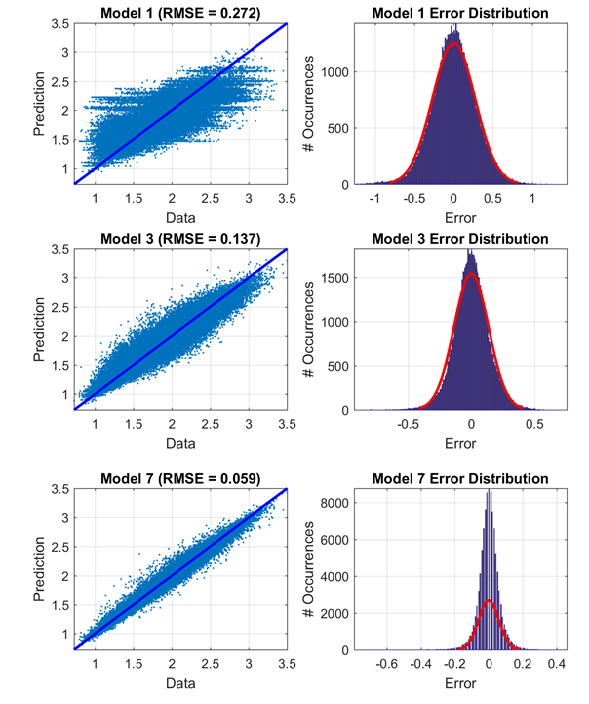
\includegraphics[scale=1.3]{Figure_1} % Include the image placeholder.png
\end{center}
\vspace*{-10mm} % Space between figure and captio
\caption{Model predictions: Left quadrants show observed vs predicted data for validation set (100,000 points) for Models 1, 3 and 7; right quadrants show histograms with corresponding error distributions for each model.}
\label{fig:MARS}
\end{figure}

\begin{figure}[!h]
\begin{center}
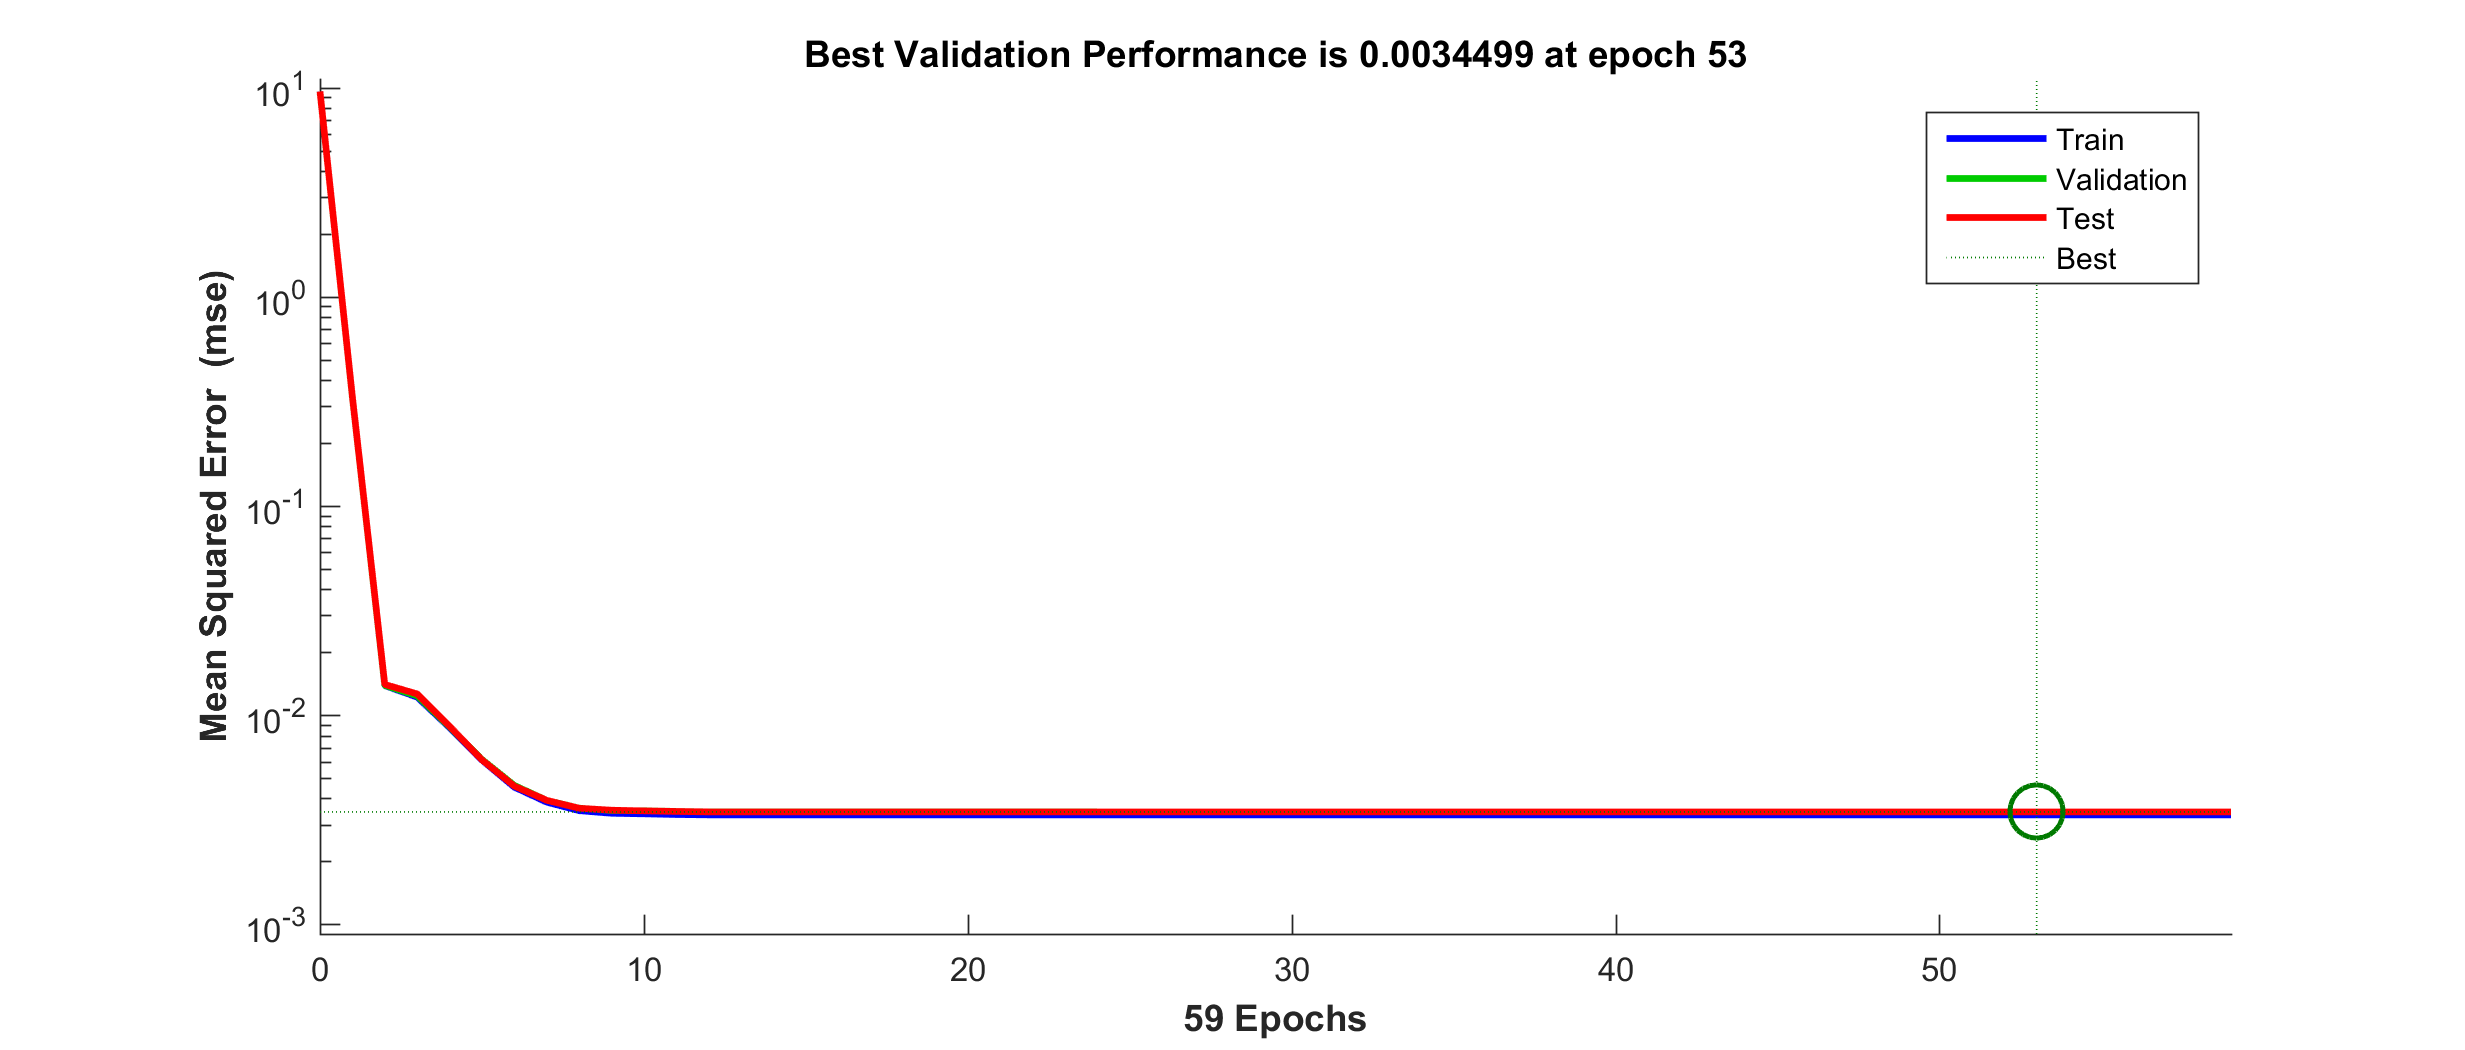
\includegraphics[scale=0.2]{Figure_2} % Include the image placeholder.png
\end{center}
\vspace*{-5mm} % Space between figure and captio
\caption{Ensemble of Models: Solution convergence using feedforward ANN with 53 epochs.}
\label{fig:Ensemble_of_Models}
\end{figure}


%----------------------------------------------------------------------------------------
%	SECTION: DISCUSSION
%----------------------------------------------------------------------------------------

\section{Discussion}

\textbf{- Application of Gradient Boosted Trees}: Analysis using XGBoost was broken down into four iterations. The first iteration made use of the relevant provided features. The model performed well as it made a slight improvement on the Random Forest baseline. As the model was trained using a comprehensive grid-search cross validation and trained on $2000$ trees, it appeared as if this competition would be won by comprehensive feature engineering rather than powerful modeling. Using the rdMolDescriptors module from RDKit, thirteen new features extracted including exact molecular weight, number of rings, among others. Our intuition was correct as adding these $13$ features drastically improved the RMSE value. The third iteration included twenty-five more features that were extracted using the same module from RDKit and the model saw a slight improvement in performance. Finally, fingerprinting feature engineering and training of subsequent model was performed on an AWS EC2 instance. This final model with more than 2000 features yielded the greatest improvement in performance.\\

\textbf{- Application of ANN and SVD}: Analysis with ANN was broken into two different studies (one with SVD and another one without SVD). As it can be see from Table~\ref{tab:RSEscores} slightly better results were obtained without the application of SVD in this particular case. What this means is that a linear projection of our set of 66 attributes into their principal components does not seem appropriate for this problem. In reality those principal components must be, by definition, linear combination of the original attributes, and it's possible that such a linear projection deteriorates the ability to build a good data-driven model during the regression phase. A data reduction approach for this problem, if any, should probably be non-linear (or start from a larger feature space). As per the application of ANN a good convergence was observed with most cases. Our scores improved once new molecular features were added on top of the baseline features. It's worth noticing that several runs were performed with ANN for different network architectures, different random subdivisions of the training data (i.e., we used a fraction of that training data to control overfitting in some cases); different approaches towards normalization of the added features were also considered. Model 2 in Table~\ref{tab:RSEscores} is a good representative model of the ANN effort. \\

\textbf{- Application of MARS}: Application of MARS was interesting here as it represents and advanced technique to fit data to a closed form (in this case splines with flexible basis functions). The run time for MARS was significantly higher than ANN (8h vs 2h respectively), and still results were slightly worse. In general ANN seems to provide better characteristics to fit the data in this problem. One of the advantages of MARS though is that there is very little need (if any) to optimize hyperparameters. \\

\textbf{- Final comments}: Based on the analysis conducted for this project it seems clear that our RMSE values could only be significantly improved after a significant number of features were generated from RDKit. This emphasizes the important of feature engineering in machine learning applications. Our best results by far were obtained when more than 2000 features were considered for the problem. The application of different regression techniques also helped us build a robust ensemble of models.

%----------------------------------------------------------------------------------------
%	BIBLIOGRAPHY
%----------------------------------------------------------------------------------------
\section*{References}
\fontsize{7pt}{7pt}\selectfont
\begin{itemize}
  \item {[1] Matlab, Neural Network toolbox, \url{http://www.mathworks.com/help}}
  \item {[2] J. H. Friedman, “Multivariate adaptive regression splines (with discussion),” Annals of Statistics, vol. 19, pp. 1–141, 1991}
	\item {[3] XGBoost, \url{https://github.com/dmlc/xgboost}}
	\item {[4] Computation of the Singular Value Decomposition, \url{http://www.cs.utexas.edu/users/inderjit/public_papers/HLA_SVD.pdf}}
  \item {[5] Montavon G., et al., "Machine Learning of Molecular Electronic Properties in Chemical Compound Space"\url{http://arxiv.org/pdf/1305.7074.pdf}}
	\item {[6] The BellKor Solution to the Netflix Grand Prize, \url{http://www.netflixprize.com/assets/GrandPrize2009_BPC_BellKor.pdf}}

\end{itemize}


%----------------------------------------------------------------------------------------
%	APPENDIX
%----------------------------------------------------------------------------------------
\section*{Appendix}
\fontsize{7pt}{7pt}\selectfont
All code from this practical can be found at the following Google Drive link: \\ \\ \url{https://drive.google.com/a/g.harvard.edu/folderview?id=0B0e1_K8CvqynMk5uWDRDNXZXTHc&usp=sharing#} \\ \\
%----------------------------------------------------------------------------------------
\end{document}